\section{Choosing a vision on the loop solution}

In order to create our embedded system, we have to follow somme specifications : 

\begin{enumerate}
 \item The system is composed by a camera mounted on two servomotors (JIWY2) and controlled by one of this setup :
 \begin{enumerate}
  \item Combination of an altera DE0-NANO and an Overo fire.
  \item RaMstix extension board for Overo FireStorm-P
 \end{enumerate}
 \item The system is able to process image form the camera and move the camera in fonction.
\end{enumerate}

In order to follow this specifications, there is several option. For example, we could have created a system that goes alternatively to differents colors or try to avoid capting a specific shape. This systems although funnier to create and use would have been more difficult to implement therefore we finally chose and easier system that consist on following a specific color shape on the picture get by the webcam to have this shape in the center of thhe picture.

\begin{figure}[!ht]
\centering
 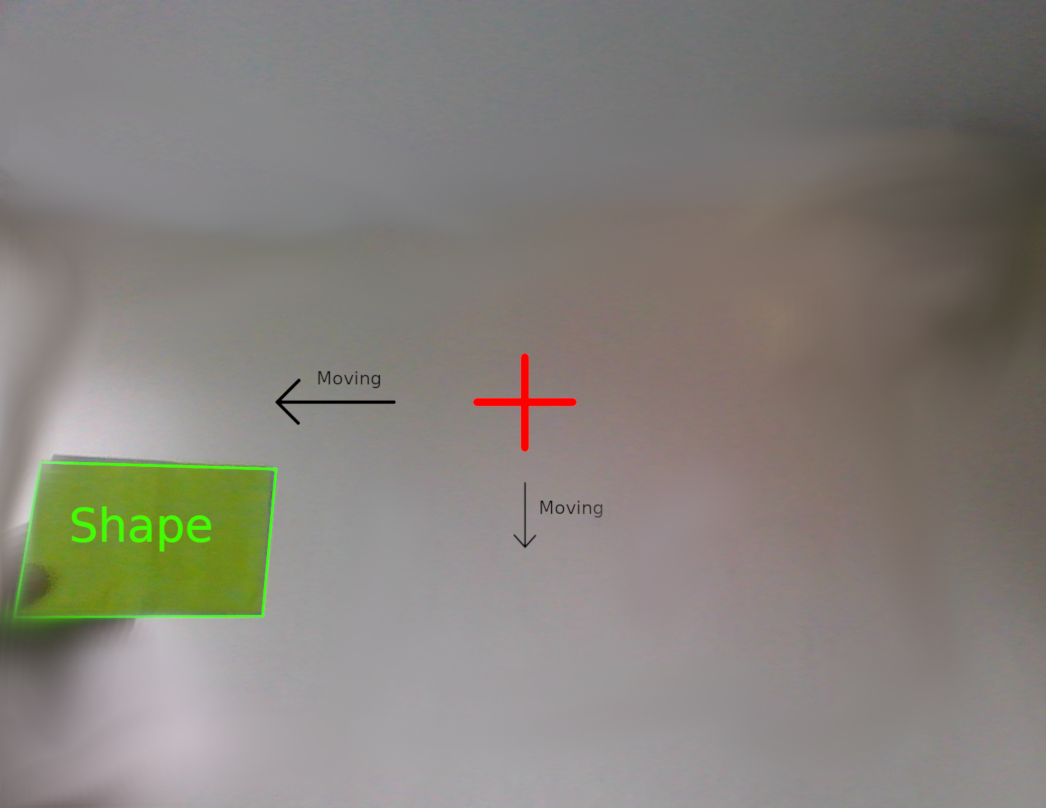
\includegraphics[width=0.5\textwidth]{visionOnTheLoop.png}
 \caption{Our vision-on-the-loop solution}
 \label{votl}
\end{figure}


